\documentclass[12pt,fleqn]{article}
\usepackage{amsfonts}
\usepackage{amsmath,amsthm,amssymb,graphicx,setspace,url,booktabs,tabularx,enumerate,slantsc}
\usepackage[T1]{fontenc}

\usepackage[sort,round,comma]{natbib}
\usepackage[margin=1.25in]{geometry}
\usepackage[small]{caption}
\usepackage[charter]{mathdesign}
\urlstyle{same}
\newcolumntype{C}{>{\centering\arraybackslash}X}
\bibliographystyle{abbrvnat}
\newcommand\citepos[2][]{\citeauthor{#2}'s \citeyearpar[#1]{#2}}
\newcommand\poscw{\citeauthor{ClW:06}'s \citeyearpar{ClW:06,ClW:07}}
\newcommand\citen[1]{\citeauthor{#1}, \citeyear{#1}}
\frenchspacing
\newcommand{\empiricalcriticalvalue}{2.67}
\newcommand{\spacriticalvalue}{1.26}
\newcommand{\nboot}{599}
\newcommand{\bootsize}{10}
\newcommand{\windowlength}{10}
\newcommand{\empiricaltable}{% latex table generated in R 3.2.0 by xtable 1.7-4 package
% Mon Apr 20 13:17:43 2015
\begin{tabularx}{\textwidth}{lCCCC}
  \toprule   & value & naive & SPA & ours \\ 
  \midrule long term rate & $\enskip1.56$ & sig. & sig. &  \\ 
  book to market & $\enskip1.41$ & sig. & sig. &  \\ 
  dividend yield & $\enskip1.27$ &  & sig. &  \\ 
  dividend price ratio & $\enskip0.95$ &  &  &  \\ 
  net equity & $\enskip0.70$ &  &  &  \\ 
  dividend payout ratio & $\enskip0.64$ &  &  &  \\ 
  treasury bill & $\enskip0.53$ &  &  &  \\ 
  stock variance & $\enskip0.50$ &  &  &  \\ 
  default return spread & $\enskip0.16$ &  &  &  \\ 
  default yield spread & $\enskip0.09$ &  &  &  \\ 
  inflation & $\!\!-0.09$ &  &  &  \\ 
  term spread & $\!\!-0.43$ &  &  &  \\ 
  earnings price ratio & $\!\!-0.56$ &  &  &  \\ 
  long term yield & $\!\!-0.74$ &  &  &  \\ 
   \bottomrule \end{tabularx}
}


% These commands are generated when the monte carlo and applied
% sections are run; I'm giving them definitions now so that LaTeX will
% run.
\providecommand\bootsize{[missing]}
\providecommand\empiricalcriticalvalue{[missing]}
\providecommand\nboot{[missing]}
\providecommand\testsize{[missing]}
\providecommand\totalsims{[missing]}
\providecommand\windowlength{[missing]}
\providecommand\empiricaltable{[missing]}

\newtheorem{thm}{Theorem}
\newtheorem{lem}[thm]{Lemma}
\newtheorem{claim}[thm]{Claim}
\newtheorem{cor}[thm]{Corollary}
\newtheorem{lema}{Lemma}[subsection]
\newtheorem{alg}{Algorithm}
\newtheorem{asmp}{Assumption}
\theoremstyle{definition}

\newtheorem{example}{Example}
\newtheorem{defn}{Definition}
\newtheorem{rem}{Remark}

\DeclareMathOperator*{\argmin}{arg\,min}
\DeclareMathOperator{\E}{E}
\DeclareMathOperator{\var}{var}
\DeclareMathOperator{\cov}{cov}
%\DeclareMathOperator{\vec}{vec}
\DeclareMathOperator{\vech}{vech}

\DeclareMathOperator{\pr}{Pr}

\newcommand{\btrue}{\beta_0}

\newcommand{\X}{\ensuremath{\mathrm{X}}}
\newcommand{\R}{\ensuremath{\mathrm{R}}}
\newcommand{\p}{\ensuremath{\mathrm{P}}}

\newcommand{\bh}{\hat \beta}
\newcommand{\ep}{\varepsilon}
\newcommand{\eph}{\hat\varepsilon}
\newcommand{\fb}{\bar f}
\newcommand{\fh}{\hat f}
\newcommand{\Hs}{\mathcal{H}}

\newcommand{\osum}[1]{\sum_{#1=R}^{T-1}}
\newcommand{\omax}[1]{\max_{#1=R,\dots,T-1}}
\newcommand{\oavg}[1]{\tfrac{1}{P} \osum{#1}}
\newcommand{\oclt}[1]{\tfrac{1}{\sqrt{P}} \osum{#1}}

\newcommand{\aic}{AIC}
\newcommand{\bic}{BIC}
\newcommand{\brc}{BRC}
\newcommand{\cdf}{CDF}
\newcommand{\clt}{CLT}
\newcommand{\dd}[1]{\frac{\partial}{\partial #1}}
\newcommand{\dgp}{DGP}
\newcommand{\fclt}{FCLT}
\newcommand{\fwe}{FWE}
\newcommand{\gdp}{GDP}
\newcommand{\gmm}{GMM}
\newcommand{\hac}{HAC}
\newcommand{\iv}{IV}
\newcommand{\lln}{LLN}
\newcommand{\ma}{MA}
\newcommand{\mds}{MDS}
\newcommand{\ned}{NED}
\newcommand{\ols}{OLS}
\newcommand{\oos}{OOS}
\newcommand{\sfwe}{SFWE}
\newcommand{\spa}{SPA}
\newcommand{\wfwe}{WFWE}

\renewcommand{\Re}{\ensuremath{\mathbb{R}}}

\renewcommand{\topfraction}{.85}
\renewcommand{\bottomfraction}{.7}
\renewcommand{\textfraction}{.15}
\renewcommand{\floatpagefraction}{.66}
\renewcommand{\dbltopfraction}{.66}
\renewcommand{\dblfloatpagefraction}{.66}
\setcounter{topnumber}{9}
\setcounter{bottomnumber}{9}
\setcounter{totalnumber}{20}
\setcounter{dbltopnumber}{9}

\date{2015-05-08}

\begin{document}

\author{Gray Calhoun\thanks{ Economics Department; Iowa State
    University; Ames, IA 50011.  Telephone: (515) 294-6271.  Email:
    \guillemotleft\protect\url{gcalhoun@iastate.edu}\guillemotright.  Web:
    \guillemotleft\protect\url{http://gray.clhn.org}\guillemotright.
    If you find an error in this paper, please let me know by email or
    by filing a new issue at
    \guillemotleft\protect\url{https://git.ece.iastate.edu/gcalhoun/oosbootstrap/issues}\guillemotright.
    I'd like to thank Helle Bunzel, Todd Clark, and Michael McCracken
    for helpful comments and discussions.  I'd also like to thank Amit
    Goyal for providing computer code and data for his 2008
    RFS paper with Ivo
    Welch \citep{GoW:08}.} \\
  Iowa State University}

\title{A simple block bootstrap for asymptotically normal
  out-of-sample test statistics}

\maketitle

\begin{abstract} \noindent%
  This paper proposes an improved block bootstrap method for
  out-of-sample statistics. Previous block bootstrap methods for these
  statistics have centered the bootstrap out-of-sample average on the
  observed out-of-sample average, which can cause the distribution to
  be miscentered under the null --- these papers have used either a
  short out-of-sample period or an adjustment to the model parameter
  estimators under the bootstrap to correct this centering
  problem. Our approach centers the bootstrap replications correctly
  under the null while continuing to use the standard formulas to
  estimate the model parameters under the bootstrap, while allowing
  the out-of-sample period to remain large. The resulting approach is
  computationally more efficient and easier to program.

\strut

\noindent Keywords: Forecast Evaluation, Martingale Difference
Sequence, Model Selection, Family-Wise Error Rate; Multiple Testing;
Bootstrap; Reality Check

\strut

\noindent JEL Classification Numbers: C22, C53

\end{abstract}

\newpage

\section{Introduction}

This paper develops a block bootstrap method that can be used to
consistently estimate the distributions of asymptotically normal
out-of-sample (\oos) test statistics. We propose the ``obvious''
approach of drawing a large number of bootstrap samples from the full
dataset --- using the Moving Blocks, Circular Block, or Stationary
bootstraps proposed by \cite{Kun:89}, \cite{LiS:92}, \cite{PoR:92},
and \cite{PoR:94} (which we will define shortly) --- and then
calculating the \oos\ statistic of interest for each bootstrap sample.
We show that this approach is valid under conditions simliar to
\citepos{Wes:96} and \citepos{Mcc:00}; i.e. when the \oos\ statistic
itself is asymptotically normal.

The block bootstraps mentioned in the previous paragraph are all
nonparametric techniques: each of these bootstraps draws $J$ blocks of
length $\ell$ at random from the original dataset, and assembles them
into a new bootstrap time-series. If $\ell \to \infty$ as $T \to
\infty$, the blocks capture the serial dependence in the original data
without any additional effort by the researcher. (Under the right
weak-dependence assumptions and other conditions on the \dgp,
obviously.) These methods differ slightly in how they conduct this
random sampling. For the \emph{Moving Blocks Bootstrap} developed by
\cite{Kun:89} and \cite{LiS:92}, $\ell$ is set by the researcher, and
each block of $\ell$ consectutive observations is equally likely to be
chosen. The same principle applies for \citepos{PoR:92} \emph{Circular
  Block Bootstrap}, but now the bootstrap is allowed to ``wrap
around'' the endpoints of the original time series and choose, for
example, the block with indices $T-1,T, 1, 2,\dots, \ell - 2$.%
\footnote{This modification ensures that the mean of the distribution
  induced by the bootstrap always equals the sample mean.} %
\citepos{PoR:94} \emph{Stationary Bootstrap} extends the Circular
Block Bootstrap by drawing the block length independently for each
block from the geometric distribution.%
\footnote{This additional source of randomization produces a strictly
  stationary bootstrap sequence. It also reduces the efficiency of the
  Stationary Bootstrap relative to the other block bootstraps, but by
  less than was originally thought. See \cite{Nor:09} for a discussion
  of this issue.}

Although the nonparametric aspect of these block boostraps has led to
their popularity in many areas of time-series econometrics, they have
been relatively unpopular in the \oos\ testing literture. This is due
to several factors. Although the first papers developing the
theoretical properties of these statistics, \cite{DiM:95} and
\cite{Wes:96}, prove asymptotic normality, subsequent papers show that
asymptotic normality tends to hold only under restrictive conditions
and fails otherwise. (See \citealp{ClM:01}, and \citealp{Mcc:07}, in
particular.) Consequently, most papers focus on misspecification tests
for nested models, where it is natural to impose that a restricted
benchmark model holds under the null hypothesis and to use that
restricted model to generate the bootstrap samples, as in
\cite{Lut:99} and \cite{ClM:05}.
However, \cite{GiW:06}, \cite{ClW:06,ClW:07}, and \cite{Cal:15} have
proposed \oos\ test statistics that are asymptotically normal under
general conditions, so it is worth exploring whether block bootstraps
can be applied to these new statistics. This is especially true since
researchers will often want to allow the benchmark model to be
misspecified under the null hypothesis in forecasting applications and
when comparing several models, which is straightforward with block
bootstraps but more difficult with parametric bootstraps. (See in
particular \citealp{Whi:00}, \citealp{Han:05}, and \citealp{RoW:05}.)

Previous treatments of these bootstraps have focused on restricted or
recentered bootstraps, but ours seems to be the first to study the
theoretical properties of a standard boostrap applied to the entire
dataset. \citet{Whi:00} and \citet{Han:05}, for example, require the
out-of-sample period to be very small relative to the total sample
size to remove the effects of estimating the unknown parameters of the
forecasting models. \cite{CoS:07} propose a different bootstrap
procedure that adds a recentering term to the parameter estimates and
the \oos\ average; these adjustments can be somewhat awkward to
implement and can add to the computation time, which reduces some of
the block bootstrap's advantages. In our paper, in contrast, we show
that standard nonparametric block bootstraps are consistent without
modification and derive the correct centering term to ensure
consistency.

The next section presents our theoretical results. Section~\ref{sec:3}
presents an empirical illustration of our approach based on
\citepos{Cal:15} \oos\ statistic, and Section~\ref{sec:mc} presents a
Monte Carlo experiment that studies the bootstrap's finite sample
properties. Finally, Section~\ref{sec:4} concludes.

\section{The Bootstrap for Out-of-Sample Statistics}

We'll develop our theoretical results in a fairly general
framework. Let $y_{t+1}$ be a target variable of interest --- a
variable that is being predicted --- and let $x_t$ be a vector of
other variables that are potentially informative about $y_{t+1}$ ---
these are our predictors. The forecast $\hat y_{t+1}$ depends on the
variables $x_t$ and an estimated parameter $\bh_t$. In the research
project that we're trying to model, we're interested in a function of
these variables and parameters, and the \oos\ average of that function
is our test statistic.

In symbols, we're interested in statistics of the form
\begin{equation*}
  \fb = \oclt{t} f(y_{t+1}, x_t, \bh_{1t},\dots,\bh_{kt})
  \equiv \oclt{t} f_t(\bh_{1t},\dots,\bh_{kt}),
\end{equation*}
where each $\bh_{kt}$ corresponds to a different forecasting model.
To make the notation cleaner, we'll define $f_t(\beta_1,\dots,\beta_k)
\equiv f(y_{t+1}, x_t, \beta_1,\dots,\beta_k)$. We're also going to
assume that $(y_{t+1}, x_t)$ is strictly stationary to simplify our
presentation. One could derive the same results under the marginally
weaker assumption that certain functions of these variables are weakly
stationary.

The coefficients are updated each period to mimic a true \oos\
forecasting exercise. In this paper, we're going to assume that each
$\bh_{it}$ is an $M$-estimator. We expect that other classes of
estimators can be used as well, as long as they are amenable to the
bootstrap.

Using standard terminology, the estimator $\bh_{it}$ is defined as
\begin{equation}\label{eq:9}
  \hat\beta_{it} = \begin{cases}
    \argmin_\beta \sum_{s=1}^{t-1} q_i(y_{s+1}, x_s, \beta) & \text{recursive window} \\
    \argmin_\beta \sum_{s=t-R+1}^{t-1} q_i(y_{s+1}, x_s, \beta) & \text{rolling window} \\
    \argmin_\beta \sum_{s=1}^{R-1} q_i(y_{s+1}, x_s, \beta) & \text{fixed window},
  \end{cases}
\end{equation}
and, as before, to make the notation cleaner, define $q_{is}(\beta)
\equiv q_i(y_{s+1},x_s,\beta)$. Obviously, for this to be a reasonable
estimation approach $q_{is}$ will need to satisfy standard assumptions
that we'll discuss soon. The implicit assumption is that the
researcher is interested in conducting inference on $\E
f_t(\beta_{10},\dots,\beta_{k0})$, where
\begin{equation*}
  \beta_{i0} = \argmin_\beta \E q_i(y_{s+1}, x_s, \beta)
\end{equation*}
is the pseudotrue equivalent of $\bh_{it}$,

So far, this is is a very standard setup. Our ``novelty'' is in how we
propose bootstrapping $\fb$. Of course, people familiar with the
bootstrap should not find it novel at all --- we use a standard block
bootstrap and replace parameters with their equivalents under the
bootstrap-induced distribution. But this is not how the bootstrap has
been applied in this literature in the past.

For the moment, consider the circular block bootstrap, which is
implemented by drawing blocks of $\ell_1$ consecutive observations
from the original dataset. For the circular block bootstrap, if the
block extends beyond the dataset it is ``wrapped around,'' so, for
example, $(T-1, T, 1, 2, 3, 4)$ is a possible block of indices when
the block length is 6.

We know from West's (1996) paper that, under appropriate assumptions,
$\sqrt{P} (\fb - \E f_t(\btrue))$ is asymptotically normal with mean
zero. The key insight in our paper is that we can match this result in
the bootstrap, but we need to be careful about the exact centering
term.  In particular, under the circular bootstrap, $\btrue^*$ is the
equivalent of $\btrue$ and the sample average is the equivalent of the
population mean. That means that we should expect
\begin{equation*}
  \sqrt{P} (\fb^* - \E^* f_t^*(\btrue^*))
\end{equation*}
to have the same asymptotic distribution and to give reliable
confidence intervals, etc. where, for the circular and stationary
block bootstraps,
\begin{equation*}
  \E^* f_t^*(\beta_1,\dots,\beta_k) = \tfrac{1}{T-1} \sum_{t=1}^{T-1} f_t(\beta_1,\dots,\beta_k)
\end{equation*}
and
\begin{equation*}
  \beta_{i0}^* = \argmin_\beta \sum_{s=1}^{T-1} q_i(y_{s+1}, x_s, \beta).
\end{equation*}
For the moving blocks bootstrap, a slight correction is necessary
since observations at the ends of the sample are less likely to be
selected, but the same equations hold approximately. And, after
spelling out our specific assumptions, that's what we'll show!

But, just to spell it out first, here
\begin{equation}
  \fb^* = \oavg{t} f(y_{t+1}^*, x_t^*, \bh_{1t}^*,\dots,\bh_{kt}^*)
  \equiv \oavg{t} f_t^*(\bh_{1t}^*,\dots,\bh_{kt}^*)
\end{equation}
where $\bh_{it}^*$ is estimated exactly the same way as $\bh_t$:
\begin{equation}\label{eq:10}
  \hat\beta_{it}^* = \begin{cases}
    \argmin_\beta \sum_{s=1}^{t-1} q_{is}^*(\beta) & \text{recursive window} \\
    \argmin_\beta \sum_{s=t-R}^{t-1} q_{is}^*(\beta) & \text{rolling window} \\
    \argmin_\beta \sum_{s=1}^{R-1} q_{is}^*(\beta) & \text{fixed window}
  \end{cases}
\end{equation}
and $q_{is}^*(\beta) \equiv q_i(y_{s+1}^*, x_s^*, \beta)$.

In general, let $\to^{p^{*}}$ and
$\to^{d^{*}}$ refer to convergence in probability or distribution
conditional on the observed data.  Similarly, $\E^{*}$, $\var^{*}$,
and $\cov^{*}$ refer to the expectation, variance, and covariance with
respect to the probability measure induced by the bootstrap, and
$y_t^{*}$, etc. is the random variable $y_t$ but under the
bootstrap-induced \cdf.

\begin{asmp}\label{a1}
  The estimators $\bh_{it}$ and $\bh_{it}^*$ are estimated as defined in
  Equations~\eqref{eq:9} and~\eqref{eq:10}. Moreover each $\beta_{i0} =
  \argmin_\beta \E\, q_{is}(\beta)$ is uniquely identified and the vector
  $(\beta_{10},\dots,\beta_{k0})$ is an element of a compact set $\Theta$.
\end{asmp}

For the next result, let $\nabla h(\beta)$ and $\nabla^2 h(\beta)$
refer to the first and second derivative of the function $h$. If
$\beta$ is a $K$-vector, $\nabla h(\beta)$ will be $K \times 1$ and
$\nabla^2 h(\beta)$ will be $K \times K$. Also let $\nabla_i h(\beta)$
refer to the $i$th element of $\nabla h(\beta)$ and $\nabla_{ij}^2
h(\beta)$ to the $(i,j)$ element of $\nabla^2 h(\beta)$.

This assumption imposes standard moment and smoothness conditions on
the underlying functions $f_t(\cdot)$ and $q_{it}(\cdot)$. It is quite
likely that these are stronger than necessary and could be weakend to
smoothness conditions on $\E f_t(\cdot)$ and $\E q_{it}(\cdot)$, as in
\cite{Mcc:00}, but we leave that for future work.%
\footnote{Extending our results in this way would be equivalent to
  extending \cite{JoD:00} in the same way, which appears feasible but
  nontrivial.} %

\begin{asmp}\label{a2}
  The functions $f_t(\beta_1,\dots,\beta_k)$ and $q_{it}(\beta)$ are
  almost surely twice continuously differentiable in an open
  neighborhood $N$ of $(\beta_{10},\dots,\beta_{k0})$ and $\E \nabla^2
  q_{it}(\beta)$ is positive definite uniformly in $N$. There also
  exists a sequence of random variables $m_t$ such that
  $\sup_{\beta \in N} |\nabla_i^2 q_{jt}(\beta)| \leq m_t$,
  $\sup_{\beta \in N} |\nabla_{ij}^2 f_t(\beta_1,\dots,\beta_k)| \leq m_t$,
  $\sup_{\beta \in N} |\nabla_i q_{jt}(\beta)| \leq m_t$, and
  $\sup_{\beta \in N} |\nabla_i f_t(\beta_1,\dots,\beta_k)| \leq m_t$
  almost surely and $\E m_t^r$ is uniformly finite, with $r > 2$
  defined further in Assumption~\ref{a3}.
\end{asmp}

The next assumptions handle weak dependence and stationarity. These
assumptions are weaker than are typically used in this literature
because of advances in the underlying \clt\ and bootstrap theory used.
For Assumption~\ref{a3}, define
\[
  g_t(\beta_0) = (f_t(\beta_0), \nabla q_{1t}(\beta_1),\dots,\nabla q_{kt}(\beta_i))'.
\]

\begin{asmp}\label{a3}
  The stochastic process $(g_t(\beta_0), vec(\nabla g_t(\beta_0)))$ is
  weakly stationary. Moreover, $(y_{t+1},x_t)$ is strong-mixing of
  size $-r/(r-2)$ or uniform mixing of size $-r/(2r-2)$ with $r>2$.
\end{asmp}

The next assumption seriously limits the practical applicability of
these results, but is difficult to relax in general. (Well, we can
relax it for nested models, but not for ``overlapping'' models.)

\begin{asmp}\label{a6}
  The asymptotic variance matrix of $\fb$ is uniformly positive definite.
\end{asmp}

Standard assumption on the relative sizes of the test and training samples.

\begin{asmp}\label{a7}
  $R, P \to \infty$ as $T \to \infty$.
\end{asmp}

Standard assumption on block length for the bootstrap.

\begin{asmp}\label{a4}
  The bootstrap sequence $(y_2^*, x_1^*),\dots,(y_T^*, x_{T-1}^*)$ is
  constructed using a moving blocks, circular blocks, or stationary
  bootstrap with block lengths drawn from the geometric distribution.
  The (expected) block length $\ell$ satisfies $\ell \to \infty$
  and $\ell/T \to 0$.
\end{asmp}

Then the main result is proving consistency of the bootstrap
distribution and the bootstrap variance.

\begin{thm}\label{res:3}
  Under Assumptions~\ref{a1} -- \ref{a4}, $\var(\fb)/\var^*(\fb^*)
  \to^p 1$ and
  \begin{equation}\label{eq:15}
    \pr\big[\sup_x \big\lvert \pr^*[\sqrt{P} (\fb^* - \E^* f_t^*) \leq x]
    - \pr[\sqrt{P}( \bar{f} - \E f_t) \leq x] \big\rvert > \epsilon\big] \to 0
  \end{equation}
  for all $\epsilon > 0$.
\end{thm}

\begin{rem}
  \citet{Mcc:00} proves asymptotic normality under weaker smoothness
  conditions on $f_t(\beta)$ and $h_t(\beta)$: only their expectations
  must be continuously differentiable.  It may be possible to extend
  Theorem~\ref{res:3} to those weaker conditions, but the current
  proof relies on a theorem of \citepos{JoD:00} establishing the
  consistency of \hac\ estimators and their theorem requires differentiability of
  the observations.  Extending \citepos{JoD:00} result to
  nondifferentiable functions should be possible, but is beyond the
  scope of this paper.
\end{rem}

\begin{rem}
  \citet{Whi:00} and \citet{Han:05} resample the forecasts but do not
  reestimate any of them which requires the additional assumption that
  $\tfrac{P}{R} \log \log R \to 0$ or that the forecasts themselves
  have no estimated parameters.%
\footnote{\citet{Whi:00} lists several
    different sets of assumptions that give the same result, but these
    seem to be the most general.} %
\end{rem}

\begin{rem}
  \citet{CoS:07} use the distribution of $\sqrt{P}(\bar{f}^{*} -
  \bar{f})$ to approximate that of $\sqrt{P}(\bar{f} - \E
  \bar{f}(\btrue))$.  But it is clear that $\bar{f}(\btrue^*)$
  is the bootstrap analogue of $\E \bar{f}(\btrue)$, the parameter of
  interest.  Because their bootstrap is miscentered, \citet{CoS:07}
  must redefine $\hat{\beta}_t^{*}$ to achieve consistency.  In this
  paper, though, consistency arises naturally.
\end{rem}

\begin{rem}
  It may be unnecessary to assume that $\bar{f}(\btrue)$ has positive
  definite asymptotic variance; if so, the bootstrap would work in the
  setup of \citet{ClM:05,ClM:01} and \citet{Mcc:07}.  That question is
  left to future research.
\end{rem}

Often economic theory will imply that $f_t$ should be a martingale
difference sequence, at least under the null hypothesis of interest.
Under this stronger null hypothesis, the bootstrap procedure can be
simplified somewhat: the bootstrap is consistent with a block length
of 1.
\begin{thm}
  Suppose that Assumptions \ref{a1} -- \ref{a7} hold and also assume
  that $f_t - \E f_t$ is an \mds\ and that the i.i.d.\ bootstrap is
  used instead of the block bootstraps of Theorem~\ref{res:3}. Then
  $\var(\fb)/\var^*(\fb^*) \to^p 1$
  and
  \begin{equation}\label{eq:20}
    \pr\big[\sup_x \big\lvert \pr^*[\sqrt{P} (\fb^* - \E^* f_t^*) \leq x]
    - \pr[\sqrt{P}( \bar{f} - \E f_t) \leq x] \big\rvert > \epsilon\big] \to 0
  \end{equation}
  for all $\epsilon > 0$.
\end{thm}
The proof is a straightforward modification of that of
Theorem~\ref{res:3} and is omitted.

\section{Empirical Illustration}\label{sec:3}

This section demonstrates the use of our new statistic by revisiting
\citepos{GoW:08} study of excess stock returns.  Goyal and Welch argue
that many variables thought to predict excess returns (measured as the
difference between the yearly log return of the S\&P 500 index and the
T-bill interest rate) on the basis of in-sample evidence fail to do so
out-of-sample.  To show this, Goyal and Welch look at the forecasting
performance of models using a lag of the variable of interest, and
show that these models do not significantly outperform the excess
return's recursive sample mean.

Here, I conduct the same analysis, but using this paper's \mds\ test.
The benchmark model is the excess return's sample mean (as in the
original) and the alternative models are of the form
\[\text{excess return}_{t} = \alpha_{0} + \alpha_{1}\
\text{predictor}_{t-1} + \varepsilon_{t},\] where $\alpha_{0}$ and
$\alpha_{1}$ are estimated by \ols\ using a \windowlength-year window.
The predictors used are listed in the ``predictor'' column of
Table~\ref{tab:em1} \citep[see][for a detailed description of the
variables]{GoW:08}.  We also consider \citepos{CaT:08} proposed
correction to the models, that the forecasts be bounded below by zero
since negative forecasts are incredible, as well as two simple
combination forecasts, the mean and the median (over both the original
and the non-negative forecasts).  The data set is annual data
beginning in 1927 and ending in 2009, and the rolling window uses
\windowlength\ observations.%
\footnote{This statistical analysis was
  conducted in R \citep{R} using the xtable
  \citep[version~1.6-0]{Dah:09}, and dbframe \citep[version
  0.2.7]{Cal:10b} packages.} %

Table~\ref{tab:em1} presents the results for each model.  The column
``value'' gives the value of the test statistic for each model, while
the ``naive'' and ``corrected'' columns indicate whether the statistic
is greater than the standard size-\bootsize\% critical value (1.28)
and the critical value estimated by the procedure of
Theorem~\ref{res:2} (\empiricalcriticalvalue).%
\footnote{The bootstrap
  uses \nboot\ replications with i.i.d. sampling, as proposed in
  conclusion~\ref{it:1} of Theorem~\ref{res:2}.} %
Three predictors are
significant at the naive critical values for both the original and
bounded forecasts: the dividend yield, long term interest rate, and
book to market ratio.  But none are significant after accounting for
data snooping, which highlights the importance of these methods.  The
median forecast is significant using conventional critical values as
well, but not the corrected values.

\begin{table}[tb!]
  \centering
  \empiricaltable
\caption{Results from \oos\ comparison of equity premium prediction
  models; the benchmark is the recursive sample mean of the equity
  premium and each alternative model is a constant and single lag of
  the variable listed in the ``predictor'' column.  The dataset begins
  in 1927 and ends in 2009 and is annual data. The ``value'' column
  lists the value of this paper's \oos\ statistic, the ``naive''
  column indicates whether the statistic is significant at standard
  critical values, and the ``corrected'' column indicates significance
  using the critical values proposed in Theorem~\ref{res:2} that
  account for the number of models.  See Section~\ref{sec:3} for details.}
\label{tab:em1}
\end{table}

\section{Monte Carlo results}\label{sec:mc}
\begin{figure}[t]
  \centering
  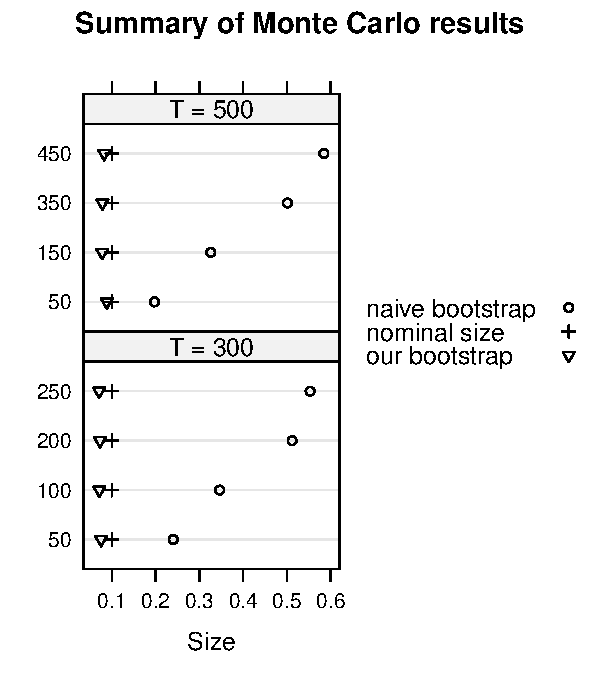
\includegraphics{montecarlo/west_iv.pdf}
  \caption{Visual summary of Monte Carlo results.}
  \label{fig:1}
\end{figure}

\section{Conclusion}\label{sec:4}
The paper improves block bootstrap procedures of \oos\
statistics.

\appendix
\section*{Appendix: Additional mathematical results}\label{sec:B}
\renewcommand{\thesubsection}{\Alph{subsection}}

We will prove our results under the simplifying assumption that there
is a single sequence of $M$-estimators $\bh_t$. Since we are assuming
non-degeneracy of the models, this assumption does not appreciably
change our arguments. This also implies that we will drop the $i$
index for the estimators $\bh_{it}$, estimation criteria
$q_{it}(\beta)$ etc.

To make the mathematical results in this appendix clearer, we will
introduce the following additional notation:
\begin{itemize}
\item $f_t = f_t(\btrue)$ and $f_t^* = f_t^*(\btrue^*)$
\item $F_t(\beta) = \nabla f_t(\beta)$ and $F_t^*(\beta) = \nabla
  f_t^*(\beta)$,
\item $F_t = F_t(\beta_0)$ and $F_t^* = F_t^*(\beta_1^*)$,
\item $F = \E F_t$ and $F^* = \E^* F_t^*$,
\item $h_t(\beta) = \nabla q_t(\beta)$ and $h_t^*(\beta) = \nabla q_t^*(\beta)$,
\item $h_t = h_t(\btrue)$ and $h_t^* = h_t^*(\btrue^*)$.
\end{itemize}
Where it is feasible, we will reuse notation from \cite{Wes:96} and
\cite{WeM:98}.

Also define
\begin{align*}
  S_{ff} &= \sum_{j=-\infty}^\infty \E f_t f_{t-j}' \\
  S_{fh} &= \sum_{j=-\infty}^\infty \E f_t h_{t-j}' \\
  S_{hh} &= \sum_{j=-\infty}^\infty \E h_t h_{t-j}',
\end{align*}
$\pi = \lim P/R$, and
\begin{align*}
  \lambda_{fh} &=
  \begin{cases}
    1 - \pi^{-1} \ln(1 + \pi) & \text{recursive window}, \pi \in (0, \infty) \\
    ?                        & \text{recursive window}, \pi = 0 \\
    ?                        & \text{recursive window}, \pi = \infty \\
    \pi / 2 & \text{rolling window}, \pi \leq 1 \\
    1 - \pi / 2 & \text{rolling window}, \pi > 1 \\
    0 & \text{fixed window},
  \end{cases} \\
  \lambda_{hh} &=
  \begin{cases}
    2 \lambda_{fh} & \text{recursive window} \\
    \pi - \pi^2/3 & \text{rolling window}, \pi \leq 1 \\
    \pi - 1/3\pi & \text{rolling window} , \pi > 1 \\
    \pi & \text{fixed window}.
  \end{cases}
\end{align*}

Also define $u_1,\dots,u_J$ to be the first period of each
block of the circular bootstrap, and, for each $j = 1,\dots,J$,
define the $\sigma$-fields
\[
\Hs_j = \sigma(u_1,\dots,u_j)
\]
and
\[
\Hs_j^* = \sigma(u_1,\dots,u_j; y_1,\dots,y_T; x_1,\dots,x_T).
\]
Also let $l = T - J \ell$ be the number of elements in the last block.

\newcommand{\WesA}[1][]{\oclt{t}
  (F_t^{#1} - \E^{#1} F_t^{#1}) B^{#1} H_t^{#1}}
\newcommand{\WesB}[1][]{\tfrac{1}{\sqrt{P}} \E^{#1} F_t^{#1} \osum{t} (B_t^{#1} -
  B^{#1}) H_t^{#1}}
\newcommand{\WesC}[1][]{\oclt{t}
  (F_t^{#1} - \E^{#1} F_t^{#1}) (B_t^{#1} - B^{#1}) H_t^{#1}}

\subsection*{Proof of Theorem~\ref{res:3}}

The proof proceeds in several steps. First, we prove via a Taylor
expansion (as in \citealp{Wes:96}) that
\begin{equation}\label{eq:23}
  \pr^*[\sqrt{p} (\fb^* - \E^* f_t^*) \leq x] \to^p \Phi(x / \sigma)
\end{equation}
where $\Phi$ is the CDF of the standard normal and $\sigma$ is a known
constant. Similar arguments directly following West's imply that
\begin{equation}\label{eq:24}
  \pr[\sqrt{p} (\fb - \E f_t) \leq x] \to^p \Phi(x / \sigma)
\end{equation}
under our assumptions, so
\begin{equation}\label{eq:25}
  \pr^*[\sqrt{p} (\fb^* - \E^* f_t^*) \leq x] \to^p
  \pr[\sqrt{p} (\fb - \E f_t) \leq x].
\end{equation}
Moreover, the assumed moment conditions ensure that the variance of
$\sqrt{P} \fb^*$ under the bootstrap distribution converges to the
variance of $\sqrt{P} \fb$. Finally, a standard argument attributed
to Poly{\`a} ensures that~\eqref{eq:15} follows
from~\eqref{eq:25}. (See the proof of Theorem~1 in \citealp{Cal:14},
for example, for an explicit statement of these final steps.)

For~\eqref{eq:23}, begin by expanding $f_t^{*}(\bh_t^*)$ around
$\btrue^*$ to get
  \begin{align*}
    \sqrt{P} (\fb^* - \E^* f_t^*)
    &= \oclt{t} (f_t^{*} - \E^* f_t^*)
     + \oclt{t} F_t^* \cdot (\bh_t^* - \btrue^*)
     + \oclt{t} w_t^* \\
    &= \oclt{t} (f_t^{*} - \E^* f_t^*)
     + F^* B^* \tfrac{1}{\sqrt{P}} \sum_{t=1}^{T-1} a_t h_t^* + o_{p^*}(1)
  \end{align*}
  where (similar to \citealp{Wes:96})
  \begin{equation*}
    w_{t} = \tfrac12 (\bh_t^* - \btrue^*)' \nabla^2 f_{t}^*(b_{t}^*) (\bh_t^* - \btrue^*),
  \end{equation*}
  \begin{equation}\label{eq:1}
    a_t =
    \begin{cases}
      \sum_{s=\max(R-1, t)}^{T-1} 1/s & \text{recursive window} \\
      \min(\tfrac{t}{R-1}, \tfrac{T - t}{R-1}, 1) & \text{rolling window} \\
      \tfrac{P}{R-1} 1\{t < R-1\} &  \text{fixed window},
    \end{cases}
  \end{equation}
  and each $b_{t}^*$ lies between $\bh_t^*$ and $\btrue^*$. The second equality holds because
  $\oclt{t} w_t^* = o_{p^*}(1)$ and
  \begin{equation*}
    \oclt{t} F_t^* \cdot (\bh_t^* - \btrue^*)
    = F^* B^* \tfrac{1}{\sqrt{P}} \sum_{t=1}^{T-1} a_t h_t^* + o_{p^*}(1),
  \end{equation*}
  both from Lemma~\ref{res:a4}.

  By Lemma~\ref{lem-clt},
  \begin{equation}\label{eq:19}
    \tfrac{1}{\sqrt{P}} \sum_{t=1}^{T-1} \begin{pmatrix}
      (f_t^* - \E^* f_t^*) 1\{t \geq R\} \\ a_t h_t^*
    \end{pmatrix} \to^{d^*}
    N\!
    \begin{pmatrix}
      \begin{pmatrix} 0 \\ 0 \end{pmatrix},
      \begin{pmatrix}
        S_{ff} & \lambda_{fh} S_{fh} \\
        \lambda_{fh} S_{fh}' &  \lambda_{hh} S_{hh}
      \end{pmatrix}
    \end{pmatrix}
  \end{equation}
  and $F^* \to^p F$ and $B^* \to^p B$ by Lemma~\ref{res:a3}, so
  \begin{equation}\label{eq:2}
    \pr^*[\sqrt{P} (\fb^* - \E^* f_t^*) < x] \to^p \Phi(x / \sigma)
  \end{equation}
  for all $x$, with
  \begin{equation*}
    \sigma^2 = S_{ff} + \lambda_{fh} (F B S_{fh} + S_{fh}' B'F') + \lambda_{hh} F B S_{hh} B' F'.
  \end{equation*}

  Normality for the original \oos\ average follows essentially the
  same argument (this is essentially the same argument as in
  \citealp{Wes:96}; the Lemmas referenced above establish intermediate
  results for the original \oos\ statistic under our assumptions as
  well as the bootstrapped statistic), so
  \begin{equation}\label{eq:3}
    \pr[\sqrt{P} (\fb - \E f_t) < x] \to \Phi(x / \sigma)
  \end{equation}
  for all $x$. As discussed above, this completes the proof.\qed

\subsection{Supporting Results}

\begin{lema}\label{res:a3}
  Under the conditions of Theorem~\ref{res:3}, $\btrue^* \to^p
  \btrue$, $B^* \to^p B$, $F^* \to^p F$.
\end{lema}

\begin{proof}[Proof of Lemma~\ref{res:a3}]
  We'll present proofs of these results for the circular block
  bootstrap; the proofs for the moving blocks and stationary
  bootstraps are similar. For $\btrue^*$, by definition $\btrue^* =
  \argmin_\beta \sum_{s=2}^T q_s(\beta)$. Our smoothness and moment conditions
  ensure that $\sum_{s=2}^T q_s(\beta)$
  obeys a uniform \lln\ and converges in probability to $\E
  q_s(\beta)$ for all $\beta \in \Theta$. Then consistency of
  $\btrue^*$ follows from, for example, Theorem~2.1 of \cite{NeM:94}.

  For $F^*$, we have
  \begin{equation*}
    \pr[|F^* - F| > \epsilon] \leq
    \pr[|F^* - F| 1\{\btrue^* \in N\} > \epsilon] + \pr[\btrue^* \notin N].
  \end{equation*}
  The second probability converges to zero by consistency of
  $\btrue^*$.  Now $F^* - F = F^* - F(\btrue^*) + F(\btrue^*) - F$,
  and $F^* - F(\btrue^*) \to^p 0$ by the uniform \lln. Choose
  $\Delta$ so that $|\beta_1 - \beta_2| < \Delta$ implies that
  $|F(\beta_1) - F(\beta_2) | < \epsilon$. Then
  \begin{equation*}
     \pr[|F(\btrue^*) - F | > \epsilon] \leq \pr[|\btrue^* - \btrue| > \Delta]
  \end{equation*}
  which converges to zero by the first part of this Lemma. The proof
  for $B^*$ is similar.
\end{proof}

\begin{lema}\label{res:a_1}
  Under the conditions of Theorem~\ref{res:3},
  \begin{gather}
    \omax{t} | \hat{\beta}_{t} - \btrue | \to^{p} 0 \label{eq:26} \\
    \omax{t}  | \hat{\beta}^{*}_{t} - \btrue^* | \to^{p^{*}} 0 \label{eq:27} \\
    \omax{t} \big\lvert - \tfrac{1}{t-1} \sum_{s=1}^{t-1} \nabla h_s(b_t) - B^{-1} \big\rvert \to^p 0 \label{eq:21}
    \intertext{and}
    \omax{t} \big\lvert -\tfrac{1}{t-1} \sum_{s=1}^{t-1} \nabla h_s^*(b_t^*) - B^{*-1} \big\rvert \to^p 0 \label{eq:22}
  \end{gather}
  where each $b_t$ is any array a.s. between $\bh_t$ and $\btrue$
  and each $b_t^*$ is any array a.s. between $\bh_t^*$ and
  $\btrue^*$.
\end{lema}
The proof of~\eqref{eq:21} follows from standard
arguments for $M$-estimators and is also omitted.
\begin{proof}[Proof of~\eqref{eq:27}]
  First, assume $t \to \infty$ as $T \to \infty$. We have $\pr^*[|
  \hat{\beta}^{*}_t - \btrue^* | > \epsilon] \to^p 0$ if $\pr[|
  \hat{\beta}^{*}_{t} - \btrue^* | > \epsilon] \to 0$. To prove this
  second convergence, we will first establish that
  \begin{equation}\label{eq:28}
    \sup_{\beta \in N} \tfrac{1}{t-1} \sum_{s=1}^{t-1} (q_s^*(\beta) - \E^*q_s^*(\beta)) \to^p 0.
  \end{equation}
  Pointwise convergence holds from the \lln\ \citep{Cal:14} and
  stochastic equitcontinuity of this function is implied by our moment
  and smoothness conditions, so~\eqref{eq:28} holds by standard
  arguments. Then given uniform convergence and identification, 
  $\pr[| \hat{\beta}^{*}_{t} - \btrue^* | > \epsilon] \to 0$ follows.

  Then extending this result to
  \begin{equation*}
    \pr[ \omax{t} | \hat{\beta}^{*}_{t} - \btrue^* | > \epsilon] \to 0
  \end{equation*}
  follows the same argument as used in Calhoun's (2014) uniform \clt.
\end{proof}

\begin{proof}[Proof of \eqref{eq:22}.]
First, observe that for any $\Delta$
\begin{align}\label{eq:18}
  \pr^*\Big[&\sup_{t = R,\dots,T-1} \big\lvert - \tfrac{1}{t} \sum_{s=1}^t \nabla h_s^*(b_t^*) - B^{*-1} \big\rvert > \Delta \Big] \\
  &\leq \pr^*\Big[\sup_{t=R,\dots,T-1} \big\lvert - \tfrac{1}{t} \sum_{s=1}^t \nabla h_s^* - B^{*-1} \big\rvert 1\{\beta_0^* \in N\}> \Delta \Big]\\
  &\quad + \pr\Big[\sup_{t=R,\dots,T-1} \big\lvert - \tfrac{1}{t} \sum_{s=1}^t (\nabla h_s^*(b_t^*) - \nabla h_s^*) \big\rvert 1\{\beta_0^* \in N,\ \bh_t^* \in N\} > \Delta \Big] \\
  &\quad + \pr[\beta_0^* \notin N] + \pr[\bh_t^* \notin N \text{ for some } t = R,\dots,T-1]
\end{align}
The last two probabilities converges to zero by
Lemma~\ref{res:a2} and by~\eqref{eq:27}.  Moreover, just as in the proof of
Theorem~\ref{res:3}, $(1/t) \sum_{s=1}^t \nabla h_s^*$ can
be reexpressed as the sum of a uniformly integrable \mds\ that obeys
a uniform \lln, so the first probability on the rhs of~\eqref{eq:18}
converges to zero. Finally, since $\nabla h_s(\beta)$ is continuous
uniformly in $N$, we can choose $\delta$ so that $|\beta_1 - \beta_2|
< \delta$ implies that $|\nabla h_s(\beta_1) - \nabla h_s(\beta_2)| < \Delta$. Then
\begin{multline*}
  \pr^*\Big[\sup_{t=R,\dots,T-1} \big\lvert - \tfrac{1}{t} \sum_{s=1}^t
  (\nabla h_s^*(b_t^*) - \nabla h_s^*) \big\rvert 1\{\beta_0^* \in N,\ \bh_t^* \in N\} > \Delta \Big]
  \leq \\
  \pr^*[\sup_{t=R,\dots,T-1}  \lvert b_t^* - \btrue^* \rvert > \delta\text{ and }
  \btrue^* \in N,\text{ and } \bh_t^* \in N \text{ for all } t = R,\dots,T-1]
\end{multline*}
which again converges to zero in probability.

Now choose $\Delta$ so that
\begin{equation*}
  - \tfrac{1}{t} \sum_{s=1}^t \nabla h_s^*(b_t) - B^{*-1} < \Delta
\end{equation*}
implies that
\begin{equation*}
\Big[- \tfrac{1}{t} \sum_{s=1}^t \nabla h_s^*(b_t)\Big]^{-1} - B^* < \epsilon.
\end{equation*}
Then
\begin{multline*}
  \pr^*\Big[\sup_{t=R,\dots,T-1} \Big\lvert\Big[- \tfrac{1}{t} \sum_{s=1}^t
  \nabla h_s^*(b_t)\Big]^{-1} - B^*\Big\rvert > \epsilon\Big] \leq \\
  \pr^*\Big[\sup_{t=R,\dots,T-1}\big\lvert - \tfrac{1}{t} \sum_{s=1}^t
  \nabla h_s^*(b_t) - B^{*-1}\big\rvert > \Delta\Big]
  \to^{p^*} 0,
\end{multline*}
completing the proof.
\end{proof}

\begin{lema}\label{res:a2}
  If $a \in [0,1/2)$ and the conditions of Theorem~\ref{res:3}
  hold, then
  \begin{gather}
    \omax{t} \big\lvert (t-1)^{a-1} \sum_{s=1}^{t-1} h_s \big\rvert \to^p 0 \label{eq:6}\\
    \omax{t} \big\lvert (t-1)^{a-1} \sum_{s=1}^{t-1} h_s^* \big\rvert \to^{p^{*}} 0 \label{eq:11}\\
    \omax{t} (t-1)^a | \hat{\beta}_{t} - \btrue | \to^{p} 0 \label{eq:12}
    \intertext{and}
    \omax{t} (t-1)^a | \hat{\beta}^{*}_{t} - \btrue^* | \to^{p^{*}} 0. \label{eq:13}
  \end{gather}
\end{lema}

\noindent%
The proofs of~\eqref{eq:6} and~\eqref{eq:12} follow the same arguments
as~\citet{Wes:96} with minor tweaks as in \citet[Lemma A.2]{Cal:15}
and are omitted. Note that~\eqref{eq:12} and~\eqref{eq:13} are
refinements of~\eqref{eq:26} and~\eqref{eq:27}; \eqref{eq:26}
and~\eqref{eq:27} establish basic consistency results using standard
arguments, and these results are used heavily in the other proofs,
but~\eqref{eq:12} and~\eqref{eq:13} strengthen those results by adding
rate of convergence conditions.

\begin{proof}[Proof of~\eqref{eq:11}.]
We will present this proof under the assumption that $h_t$ is
univariate to reduce the notational clutter. Otherwise the argument
holds element-by-element.

Let $\delta$ be a positive number less than $1/2 - a$ and
define
$H_i^* = \sum_{t=K_{i-1}+1}^{K_i} h_t^*/t^{1-\delta}$, so
\begin{align*}
  \omax{t} \big| \tfrac{1}{t-1} \sum_{s=1}^{t-1} h_t^* \big|
  &\leq R^{-\delta} \max_{j=j^*_R,\dots,J} \big| \sum_{i=1}^{j} H_i^* \big|
  + R^{-\delta} \omax{t} \big| \sum_{s=K_{j^*_{t - 1}}+1}^{t-1} h_s^* / (t-1)^{1-\delta} \big|,
\end{align*}
where $j_s^*$ is defined to be the index of the block containing
observation $s$ of the bootstrap sequence.  (So, for example, $j_1^* =
1$.) Now observe that $\{H_i^*, \Hs_i^*\}$ is a martingale difference
sequence, so the maximal inequality implies that
\begin{equation*}
  \pr^*\Big[ \max_{j=j^*_R,\dots,J} \big| \sum_{i=1}^{j} H_{i}^* \big| > \epsilon \Big]
  \leq (1/\epsilon^2) \sum_{i=1}^J \E^*(H_{i}^{*2} \mid \Hs_{i-1}^*).
\end{equation*}
By definition
\begin{align*}
  \E^*(H_i^{*2} \mid \Hs_{i-1}^*)
  &= \tfrac{1}{T-1} \sum_{u = 0}^{T-2}
  \Big[\sum_{t = 1}^{\ell} h_{u + t}(\btrue^*) / (K_{i-1} + t)^{1-\delta} \Big]^2 \\
  &= \tfrac{1}{T-1} \sum_{u = 0}^{T-2} \Big[\sum_{t = 1}^{\ell}
  (h_{u + t} + h_{u + t}(\btrue^*) - h_{u + t})/ (K_{i-1} + t)^{1-\delta}\Big]^2.
\end{align*}
Since $R^{-\delta} \to 0$, to prove~\eqref{eq:11} it suffices to show that
\begin{gather}
  \tfrac{1}{T-1} \sum_{u = 0}^{T-2} \sum_{i=1}^J \Big[\sum_{t = 1}^{\ell_{i}}
  h_{u + t}/ (K_{i-1} + t)^{1-a-\delta} \Big]^2 = O_p(1) \label{eq:4} \\
  \tfrac{1}{T-1} \sum_{u = 0}^{T-2} \sum_{i=1}^J
  \sum_{t = 1}^{\ell_{i}} \big[(h_{u + t}(\btrue^*) - h_{u + t}) / (K_{i-1} + t)^{1-a-\delta}\big]^2 = O_p(1)
  \label{eq:5}
  \intertext{and}
  \omax{t} \big| \sum_{s=K_{j^*_{t - 1}}+1}^{t-1} h_s^*/(t-1)^{1-a-\delta} \big| = O_{p^*}(1).\label{eq:14}
\end{gather}
As in \citet{Cal:15}, our assumptions ensure that $h_t$ is an
$L_2$-mixingale of size $-1/2$. And if $c_t$ and $\zeta_j$ denote its
mixingale constants and coefficients, $h_t/t^{1-a-\delta}$ is also an
$L_2$-mixingale of size $-1/2$ with constants $c_t/t^{1-a-\delta}$.

For~\eqref{eq:14}, we have
\begin{align*}
  \E^* \big(\omax{t} &\big|\sum_{s=K_{j^*_t - 1}+1}^t h_s^*/(t-1)^{1-a-\delta} \big|\big)^2 \\
  &\leq \E^* \sum_{i=1}^{J} \max_{t = K_{i-1}+1,\dots,K_i} \big| \sum_{s=K_{i-1}+1}^t h_s^*/(t-1)^{1-a-\delta} \big|^2 \\
  &= O_p\Big(\tfrac{1}{T-1} \sum_{i=1}^{J} \sum_{u=0}^{T-2} \max_{t = K_{i-1}+1,\dots,K_i} \big| \sum_{s=K_{i-1}+1}^t h_{s+u} /(t-1)^{1-a-\delta} \big|^2 \\
  &\quad+ \tfrac{1}{T-1} \sum_{i=1}^{J} \sum_{u=0}^{T-2} \max_{t = K_{i-1}+1,\dots,K_i} \big| \sum_{s=K_{i-1}+1}^t (h_{s+u}(\btrue^*) - h_{s+u}) /(t-1)^{1-a-\delta} \big|^2\Big).
\end{align*}
\citepos{Mcl:75} maximal inequality for mixingales implies that
\begin{equation*}
  \E \max_{t = K_{i-1}+1,\dots,K_i} \big| \sum_{s=K_{i-1}+1}^t h_{s+u} /(t-1)^{1-a-\delta} \big|^2
  \leq \E \big| \sum_{s=K_{i-1}+1}^{K_i} h_{s+u} /(s-1)^{1-a-\delta} \big|^2.
\end{equation*}
Moreover,
\begin{multline*}
  \tfrac{1}{T-1} \sum_{i=1}^{J} \sum_{u=0}^{T-2} \max_{t = K_{i-1}+1,\dots,K_i} \big| \sum_{s=K_{i-1}+1}^t (h_{s+u}(\btrue^*) - h_{s+u}) /(t-1)^{1-a-\delta} \big|^2 \\
  \leq \tfrac{1}{T-1} \sum_{i=1}^{J} \sum_{u=0}^{T-2} \sum_{s=K_{i-1}+1}^{K_i} \big[(h_{s+u}(\btrue^*) - h_{s+u})/(t-1)^{1-a-\delta}\big]^2,
\end{multline*}
so the net result is that~\eqref{eq:14} holds whenever~\eqref{eq:4}
and~\eqref{eq:5} do.

We'll prove~\eqref{eq:4} first. Using \citepos{Mcl:75} maximal
inequality (again) implies that
\begin{align*}
  \E\Big|\tfrac{1}{T-1}
  &\sum_{u = 0}^{T-2} \sum_{i=1}^J \Big[\sum_{t = 1}^{\ell} h_{u + t}/ (K_{i-1} + t)^{1-a-\delta}\Big]^2 \Big| \\
  &= \tfrac{1}{T-1} \sum_{u = 0}^{T-2} \sum_{i=1}^J \E \Big[\sum_{t = 1}^{\ell} h_{u + t}(\btrue)/ (K_{i-1} + t)^{1-a-\delta} \Big]^2 \\
  &= O\big(\tfrac{1}{T-1}\big) \sum_{u = 0}^{T-2} \sum_{i=1}^J \sum_{t = 1}^{\ell} (K_{i-1} + t)^{2a + 2\delta-2} \\
  &= O(1) \sum_{t=1}^{T-1} t^{2a+2\delta-2}.
\end{align*}
Since $\delta$ was chosen to ensure that $2a+2\delta-2 < -1$, this
last summation is finite as required.

For~\eqref{eq:5}, expanding $h_{u+t}(\btrue^*)$ around $\btrue$ gives
\begin{align*}
  \tfrac{1}{T-1} & \sum_{u = 0}^{T-2} \sum_{i=1}^J \Big(\sum_{t = 1}^{\ell} (h_{u + t}(\btrue^*) - h_{u + t}(\btrue))/ (K_{i-1} + t)^{1-a-\delta} \Big)^2 \\
  &= \tfrac{1}{T-1} \sum_{u = 0}^{T-2} \sum_{i=1}^J \Big(\sum_{t = 1}^{\ell}
  \nabla h_{u + t}(b_{u+t}) \cdot (\btrue^* - \btrue) / (K_{i-1} + t)^{1-a-\delta}\Big)^2 \\
  &= (\btrue^* - \btrue)' \Big[\tfrac{1}{T-1} \sum_{u = 0}^{T-2} \sum_{i=1}^J \sum_{s,t = 1}^{\ell}
  \big(\tfrac{1}{(K_{i-1} + s) (K_{i-1} + t)}\big)^{1-a-\delta} \nabla h_{u + t}(b_{u+t}) \nabla h_{u + s}(b_{u+s})' \Big] (\btrue^* - \btrue) \\
  &= O_p\big(\tfrac{1}{T^2}\big) \sum_{u = 0}^{T-2} \sum_{i=1}^J \sum_{s,t = 1}^{\ell}
  \big(\tfrac{1}{(K_{i-1} + s) (K_{i-1} + t)}\big)^{1-a-\delta} \nabla h_{u + t}(b_{u+t})' \nabla h_{u + s}(b_{u+s})
\end{align*}
where each $b_{u+t}$ lies between $\btrue^*$ and $\btrue$ almost surely, and so
\begin{align*}
  \pr\Big[& \tfrac{1}{T-1} \sum_{u = 0}^{T-2} \sum_{i=1}^J
  \Big(\sum_{t = 1}^{\ell} (h_{u + t}(\btrue^*) - h_{u + t})/ (K_{i-1} + t)^{1-a-\delta}\Big)^2 > \epsilon \Big] \\
  & \leq \pr\Big[ \tfrac{1}{T^2} \sum_{u = 0}^{T-2} \sum_{i=1}^J \sum_{s,t = 1}^{\ell}
  \big\lvert \big(\tfrac{1}{(K_{i-1} + s) (K_{i-1} + t)}\big)^{1-a-\delta}
  \nabla h_{u + t}(b_{u+t})' \nabla h_{u + s}(b_{u+s}) \big\rvert 1\{\btrue^* \in N\} > \epsilon \Big] \\
  &\quad + \pr[\btrue^* \notin N].
\end{align*}
The second probability, $\pr[\btrue^* \notin N]$, converges to zero by
Lemma~\ref{res:a3}. For the first, we have
\begin{align*}
  \E \tfrac{1}{T^2} &\sum_{u = 0}^{T-2} \sum_{i=1}^J \sum_{s,t = 1}^{\ell}
  \big\lvert \big(\tfrac{1}{(K_{i-1} + s) (K_{i-1} + t)}\big)^{1-a-\delta}
  \nabla h_{u + t}(b_{u+t})' \nabla h_{u + s}(b_{u+s}) \big\rvert 1\{\btrue^* \in N\} \\
  &\leq \tfrac{1}{T^2} \sum_{u = 0}^{T-2} \sum_{i=1}^J \sum_{s,t = 1}^{\ell}
  \E \sup_{\beta \in N} \big\lvert \big(\tfrac{1}{(K_{i-1} + s) (K_{i-1} + t)}\big)^{1-a-\delta}
  \nabla h_{u + t}(\beta)' \nabla h_{u + s}(\beta) \big\rvert \\
  &\leq O(\tfrac{1}{T^2}) \sum_{u = 0}^{T-2} \sum_{i=1}^J \sum_{s,t = 1}^{\ell}
  \big(\tfrac{1}{(K_{i-1} + s) (K_{i-1} + t)}\big)^{1-a-\delta} \E | m_{u+t} m_{u+s} | \\
  &\leq O(\tfrac{1}{T^2}) \sum_{u=0}^{T-2} \sum_{i=1}^J \sum_{s = 1}^{\ell} (K_{i-1} + s)^{2a + 2\delta - 2} \E m_{u+s}^2
\end{align*}
where the second inequality holds by assumption and the third follows
from repeated application of the Cauchy-Schwarz inequality. Since $\E
m_{u+s}^2$ is bounded, the large summation is $O(T)$ and this final
term converges to zero, completing the proof.
\end{proof}

\begin{proof}[Proof of~\eqref{eq:13}.]
Expanding $h_t^*(\bh_t^*)$ around $\btrue^*$ gives
\begin{equation*}
\bh_t^* - \btrue^* = \Big(- \sum_{s=1}^{t-1} \nabla h_s^*(b_s^*) \Big)^{-1} \sum_{s=1}^{t-1} h_s^* / (t-1)
\end{equation*}
with each $b_s^*$ a.s. between $\bh_t^*$ and $\btrue^*$. Then
\begin{multline}
  \omax{t} (t-1)^a | \hat{\beta}_t - \btrue |
  \leq
  \omax{t,u} \Big|\Big[ \Big(\sum_{s=1}^{t-1} \nabla h_s^*(b_s^*) \Big)^{-1} - B^* \Big]
  (t-1)^{a-1} \sum_{s=1}^{t-1} h_s^* \Big|\\
  + \omax{t} \big| B^*   (t-1)^{a-1} \sum_{s=1}^{t-1} h_s^* \big|
\end{multline}
and both terms converge to zero in (conditional) probability by the
previous arguments.
\end{proof}

\begin{lema}\label{res:a4}
  Under the conditions of Theorem~\ref{res:3},
  \begin{equation}\label{eq:16}
    \oclt{t} (\bh_t^* - \btrue^*)' \nabla^2 f_{it}^*(b_{it}^*) (\bh_t^* - \btrue^*) \to^{p^*} 0
  \end{equation}
  and
  \begin{equation}\label{eq:17}
    \oclt{t} F_t^* \cdot (\bh_t^* - \btrue^*)
    = F^* B^* \tfrac{1}{\sqrt{P}} \sum_{t=1}^{T-1} a_t h_t^* + o_{p^*}(1).
  \end{equation}
\end{lema}

\begin{proof}[Proof of~\eqref{eq:16}]
We have
\begin{align*}
  \pr\Big[& \big|\oclt{t} (\bh_t^* - \btrue^*)' \nabla^2 f_{it}^*(b_{it}^*) (\bh_t^* - \btrue^*) \big| > \epsilon \Big] \\
  &\leq \pr\Big[1\{\btrue^* \in N, \bh_t^* \in N\ \text{for all}\ t\} \big|\oclt{t} (\bh_t^* - \btrue^*)' \nabla^2 f_{it}^*(b_{it}^*) (\bh_t^* - \btrue^*) \big| > \epsilon \Big] \\
  &\quad + \pr[\btrue^* \notin N] + \pr[\bh_t^* \notin N\ \text{for some}\ t = R,\dots,T-1\}
\end{align*}
The second two probabilities on the rhs converge to zero by
Lemma~\ref{res:a2} and the random variable inside the first probability is bounded by
\begin{multline*}
  1\{\btrue^* \in N, \bh_t^* \in N\ \text{for all}\ t\}
  \oclt{t} (\bh_t^* - \btrue^*)' \nabla^2 f_{it}^*(b_{it}^*) (\bh_t^* - \btrue^*)
  \\ \leq
  \big(\sup_{t=R,\dots,T-1} |P^{1/4}(\bh_t^* - \btrue^*)|^2\big) \oavg{t}  \nabla^2 f_{it}^*(b_{it}^*) 1\{\btrue^* \in N, \bh_t^* \in N\}.
\end{multline*}
The summation is $O_p(1)$ by assumption and the supremum converges to
zero by using Lemma~\ref{res:a2} again.
\end{proof}
\begin{proof}[Proof of~\eqref{eq:17}]
For~\eqref{eq:17}, we have the upper bound
\begin{multline*}
  \big\lvert \oclt{t} \big(F_t^* \cdot (\bh_t^* - \btrue^*) - F^* B^* a_t h_t^*\big) \big\rvert \leq \\
   \sup_{s=R,\dots,T-1} |\bh_s^* - \btrue^*|\; \big\lvert \oclt{t} (F_t^* - F^*) \big\rvert
  + \big\lvert F^* \oclt{t} \big((\bh_t^* - \btrue^*) - B^* a_t h_t^*\big) \big\rvert.
\end{multline*}
The first term converges in conditional probability to zero by
Lemma~\ref{res:a2}.

For the second, expand each $\sum_{s=1}^t \nabla q_s^*(\bh_t^*)$
around $\btrue^*$ to get
\begin{equation*}
  \oclt{t} (\bh_t^* - \btrue^*)
  = \oclt{t} \Big[\tfrac{1}{t} \sum_{s=1}^t \nabla^2 q_s^*(b_t^*)\Big]^{-1} \tfrac{1}{t} \sum_{s=1}^t h_s^*
\end{equation*}
where $b_t^*$ is between $\bh_t^*$ and $\btrue^*$. Then
\begin{align*}
  \big\lvert \oclt{t} \big((\bh_t^* - \btrue^*) - B^* a_t h_t^*\big) \big\rvert
  &\leq \sup_{t=R,\dots,T-1} \Big\lvert\Big[\tfrac{1}{t} \sum_{s=1}^t \nabla^2 q_s^*(b_t)\Big]^{-1} - B^*\Big\rvert
  \Big\lvert\oclt{t} \tfrac{1}{t} \sum_{s=1}^t h_s^* \Big\rvert \\
  &= O_{p^*}(1) \sup_{t=R,\dots,T-1} \Big\lvert\Big[\tfrac{1}{t} \sum_{s=1}^t \nabla^2 q_s^*(b_t)\Big]^{-1} - B^*\Big\rvert
\end{align*}
by Lemma~\ref{res:a2} and the supremum converges to zero in
probability by Lemma~\ref{res:a2} as well.
\end{proof}

\begin{lema}\label{lem-clt}
  Under the conditions of Theorem~\ref{res:3}, \eqref{eq:19} holds.
\end{lema}
\begin{proof}

  We will use arguments very similar to \cite{Cal:14}. Define
  \[
  \zeta_{st}^* = \gamma_1'(f_t^* - \E^* f_t^*) + a_s \gamma_2' h_t^*
  \]
  where $\gamma_1$ and $\gamma_2$ are arbitrary nonzero vectors, and
  also define
  \[
  z_j^* = \tfrac{1}{\sqrt{P}} \sum_{s=(j-1) \ell + 1}^{j\ell} \zeta_s^*
  \]
  and
  \[
  v^{*2} = J \var^*(z_j^*)
  \]
  where $\gamma = (\gamma_1', \gamma_2')'$. By construction, $\E^*
  h_t^* = 0$ almost surely, so $\E(z_j \mid \Hs_{j-1}^*) = 0$ almost
  surely and $\{z_j^*, \Hs_j^*\}$ is a martingale difference sequence.

  From the \mds\ property, we have
  \begin{equation*}
    \sum_{j=1}^J z_j^* / \sqrt{v^*} \to^d N(0, 1)
  \end{equation*}
  as long as the following properties hold:
  \begin{equation}\label{eq:7}
    \sum_{j=1}^J \E^*(z_j^{*2} 1\{z_j^{*2} > \epsilon\} \mid \Hs_{j-1}^*) \to^p 0
  \end{equation}
  and
  \begin{equation}\label{eq:8}
    \pr^*\Big[ \big| \sum_{j=1}^J z_j^{*2}/v^{*2} - 1 \big| > \epsilon\Big] \to^p 0.
  \end{equation}

  For~\eqref{eq:8}, we have the usual bound
  \begin{equation*}
    \pr^*\Big[ \big|\sum_{j=1}^J z_j^{*2}/v^{*2} - 1 \big| > \varepsilon\Big] \leq
    \pr^*\Big[ 1\{\btrue^* \in N\} \big| \sum_{j=1}^J z_j^{*2}/v^{*2} - 1 \big| > \epsilon \Big]
     + \pr^*[ \btrue^* \notin N ]
  \end{equation*}
  and we can rewrite the summation in the first term as
  \begin{equation*}
    1\{\btrue^* \in N\} \Big( \sum_{j=1}^J z_j^{*2}/v^{*2} - 1 \Big)
    =  \sum_{j=1}^J \big(1\{\btrue^* \in N\}z_j^{*2}/v^{*2} -
    \E(1\{\btrue^* \in N\}z_j^{*2}/v^{*2} \mid \Hs_{j-1}^*) \big).
   \end{equation*}
   This term is the sum of a uniformly integrable martingale
   difference sequence and satisfies the \lln\ (i.e. Davidson's, 1994,
   Theorem 19.7), and so it converges in (conditional) probability to
   zero.  The second term converges in probability to zero by
   consistency of $\btrue^*$ (Lemma~\ref{res:a3}).

   Similary, \eqref{eq:7} holds if
   \begin{equation*}
     1\{\beta_0^* \in N\} \sum_{j=1}^J \E^*(z_j^{*2} 1\{z_j^{*2} > \epsilon\} \mid \Hs_{j-1}^*) \to 0,
   \end{equation*}
   which holds by uniform integrability of $1\{\beta_0^* \in N\} z_j^{*2}$.

   Finally, since the variance of the bootstrapped statistic is
   equivalent to a \hac\ estimator,
   \begin{equation*}
     v^{*2} \to^p \gamma_1' S_{ff} \gamma_1 + 2 \lambda_{fh} (\gamma_2' S_{fh}' \gamma_1)
     + \lambda_{hh} \gamma_2' S_{hh} \gamma_2
   \end{equation*}
   holds by Theorem 2.2 of \cite{JoD:00}, using West's (1996)
   arguments to handle the $a_s$ terms.
\end{proof}

\bibliography{texextra/references}
\end{document}

% LocalWords:  ClW JEL ISI Google GiW Mcc ClM CoS CCS StW IMA GiR WeM fh X'X hh
% LocalWords:  PaT AllRefs isi ima uc sv PeT GoW lm il GoK RoW Econometrica PoR
% LocalWords:  Finan StepM studentizing studentization Whi HuW RSW recentering
% LocalWords:  DiM LiS Kun McCracken lt filtrations GoJR JoD McCracken's Econom
% LocalWords:  Corradi unstudentized studentized fg gg GoJ gcalhoun HLN li PoW
% LocalWords:  Econometricians reestimate PPW resample miscentered AnG eq Helle
% LocalWords:  Bunzel Yu Hsu Pincheira HHK th AtO ik DoH Wolak's Wol stepdown
% LocalWords:  Hsu's iq mk Ames Amit Goyal rfs Ivo Welch Wes covariance MeR McW
% LocalWords:  familywise prespecified CoD Gia pointwise misspecified InK MeP
% LocalWords:  VeR xtable Dah dbframe oos parametrizations iid dgp return's CaT
% LocalWords:  outperformance Hmisc Har nondifferentiable bT jt Meng
% LocalWords:  stationarity mixingale mixingales texextra Timmermann